% ============================================================================
% ASRI: An Aggregated Systemic Risk Index for Cryptocurrency Markets
% ============================================================================
% A Unified Framework for Monitoring DeFi-TradFi Interconnection Risk
% Authors: Murad Farzulla, Andrew Maksakov
% Organization: Resurrexi Labs / Farzulla Research
% Version: 1.0.0
% Date: December 2025
% ============================================================================

\documentclass[11pt,twocolumn]{article}

% ============================================================================
% PACKAGE IMPORTS
% ============================================================================

% Page geometry and layout
\usepackage[a4paper, margin=1in]{geometry}
\usepackage{setspace}

% Fonts and typography
\usepackage[T1]{fontenc}
\usepackage{lmodern}

% Graphics and figures
\usepackage{graphicx}
\usepackage{float}
\graphicspath{{figures/}}

% Tables
\usepackage{booktabs}
\usepackage{array}
\usepackage{longtable}
\usepackage{tabularx}
\usepackage{multirow}

% Math packages
\usepackage{amsmath}
\usepackage{amssymb}
\usepackage{amsthm}

% Bibliography
\usepackage[round,authoryear]{natbib}
\bibliographystyle{plainnat}

% Colors
\usepackage{xcolor}
\definecolor{farzullaburgundy}{RGB}{128,0,32}
\definecolor{zenodoblue}{RGB}{0,123,255}
\definecolor{orcidgreen}{RGB}{166,206,57}

% Colored boxes
\usepackage{tcolorbox}

% TikZ for custom graphics
\usepackage{tikz}
\usetikzlibrary{shapes,arrows,positioning,calc}
\usepackage{scalerel}

% Hyperlinks and PDF metadata
\usepackage{url}
\usepackage[colorlinks=true,
            linkcolor=farzullaburgundy,
            citecolor=farzullaburgundy,
            urlcolor=farzullaburgundy,
            breaklinks=true,
            pdftitle={ASRI: An Aggregated Systemic Risk Index for Cryptocurrency Markets},
            pdfauthor={Murad Farzulla, Andrew Maksakov},
            pdfkeywords={systemic risk, cryptocurrency, DeFi, stablecoin, contagion, risk index}]{hyperref}

% Allow URLs to break at hyphens and slashes
\def\UrlBreaks{\do\/\do-\do_}
\expandafter\def\expandafter\UrlBreaks\expandafter{\UrlBreaks\do\a\do\b\do\c\do\d\do\e\do\f\do\g\do\h\do\i\do\j\do\k\do\l\do\m\do\n\do\o\do\p\do\q\do\r\do\s\do\t\do\u\do\v\do\w\do\x\do\y\do\z}

% Section spacing and formatting
\usepackage{titlesec}
\titlespacing*{\section}{0pt}{1.5ex plus 0.5ex minus 0.2ex}{1ex plus 0.2ex}
\titlespacing*{\subsection}{0pt}{1.2ex plus 0.4ex minus 0.2ex}{0.8ex plus 0.2ex}

% Burgundy section headings
\titleformat{\section}{\normalfont\large\bfseries\color{farzullaburgundy}}{\thesection}{0.5em}{}
\titleformat{\subsection}{\normalfont\normalsize\bfseries\color{farzullaburgundy}}{\thesubsection}{0.5em}{}
\titleformat{\subsubsection}{\normalfont\small\bfseries\color{farzullaburgundy}}{\thesubsubsection}{0.5em}{}

% Footer customization
\usepackage{fancyhdr}

% Absolute positioning for corner logos
\usepackage{eso-pic}

% ============================================================================
% CUSTOM COMMANDS
% ============================================================================

% ORCID icon
\newcommand{\orcidicon}{\scalerel*{
    
\begin{tikzpicture}[x=3ex,y=3ex]
    \draw[fill=orcidgreen] (0,0) circle (0.5);
    \draw[white,line width=0.08ex] (0,0.15) -- (0,0.3);
    \draw[white,line width=0.08ex] (-0.15,0) -- (-0.3,0);
    \end{tikzpicture}
}{\textrm{I}}}

% Farzulla Research logo (fallback to text if image not available)
\newcommand{\farzullalogo}{%
    \IfFileExists{farzulla-logo.pdf}{%
        \href{https://farzulla.org}{\includegraphics[height=4ex]{farzulla-logo.pdf}}%
    }{%
        \href{https://farzulla.org}{\textcolor{farzullaburgundy}{\textsc{FR}}}%
    }%
}

% Version info
\newcommand{\paperver}{1.0.0}
\newcommand{\paperdate}{December 2025}
\newcommand{\paperdoi}{10.5281/zenodo.17918239}

% Metadata box
\newcommand{\metadatabox}[1]{%
\begin{tcolorbox}[
    colback=gray!5,
    colframe=farzullaburgundy,
    title=Publication Metadata,
    fonttitle=\bfseries,
    coltitle=white,
    colbacktitle=farzullaburgundy,
    width=\columnwidth,
    arc=2mm,
    boxrule=0.8pt
]
\small
\textbf{DOI:} \href{https://doi.org/#1}{\texttt{#1}}\\
\textbf{Version:} \paperver\\
\textbf{Date:} \paperdate\\
\textbf{License:} CC-BY-4.0\\
\textbf{Status:} Methodology Preprint (Empirical validation forthcoming)
\end{tcolorbox}
}

% ============================================================================
% HEADER AND FOOTER CONFIGURATION
% ============================================================================

\pagestyle{fancy}
\fancyhf{}

\fancyhead[L]{\small\href{https://farzulla.org}{farzulla.org}}
\fancyhead[R]{\small\href{https://doi.org/\paperdoi}{DOI: \paperdoi}}

\fancyfoot[C]{\small\thepage}
\fancyfoot[L]{\small Farzulla \& Maksakov}
\fancyfoot[R]{\small v\paperver~| \paperdate}

\renewcommand{\headrulewidth}{0.4pt}
\renewcommand{\footrulewidth}{0.4pt}

\fancypagestyle{firstpage}{
  \fancyhf{}
  \fancyfoot[C]{\small\thepage}
  \fancyfoot[L]{\small Farzulla \& Maksakov}
  \fancyfoot[R]{\small v\paperver~| \paperdate}
  \renewcommand{\headrulewidth}{0pt}
  \renewcommand{\footrulewidth}{0.4pt}
}

% ============================================================================
% DOCUMENT BODY
% ============================================================================

\begin{document}

% Single-column frontmatter
\onecolumn
\setstretch{1.2}
\thispagestyle{firstpage}

% Preprint status
\begin{center}
{\small\color{farzullaburgundy}\textbf{PREPRINT v\paperver} | \color{gray}Not peer-reviewed | Empirical validation forthcoming}
\end{center}
\vspace{0.5em}

% Title
\begin{center}
{\Large\bfseries ASRI: An Aggregated Systemic Risk Index for Cryptocurrency Markets}\\[0.5em]
{\large\itshape A Unified Framework for Monitoring DeFi-TradFi Interconnection Risk}\\[1em]
{\bfseries Murad Farzulla}\textsuperscript{1,2} \href{https://orcid.org/0009-0002-7164-8704}{\orcidicon\ \texttt{0009-0002-7164-8704}}\\[0.3em]
{\bfseries Andrew Maksakov}\textsuperscript{1} \href{mailto:andrew@resurrexi.io}{\texttt{andrew@resurrexi.io}}\\[0.5em]
{\small\itshape \textsuperscript{1}\href{https://resurrexi.io}{Resurrexi Labs}, \textsuperscript{2}\href{https://farzulla.org}{Farzulla Research}}\\[0.3em]
{\small \paperdate}\\[0.5em]
{\small Correspondence: \href{mailto:murad@farzulla.org}{murad@farzulla.org}}
\end{center}

% Abstract
\begin{abstract}
\noindent Cryptocurrency markets have grown to represent over \$3 trillion in capitalization, yet no unified index exists to monitor the systemic risks arising from the interconnection between decentralized finance (DeFi) protocols and traditional financial institutions. This paper introduces the Aggregated Systemic Risk Index (ASRI), a composite measure comprising four weighted sub-indices: Stablecoin Concentration Risk (30\%), DeFi Liquidity Risk (25\%), Contagion Risk (25\%), and Regulatory Opacity Risk (20\%). We derive theoretical foundations for each component, specify quantitative formulas incorporating data from DeFi Llama, Federal Reserve FRED, and on-chain analytics, and outline a comprehensive validation framework against historical crisis events including the Terra/Luna collapse (May 2022), the Celsius/3AC contagion (June 2022), and the FTX bankruptcy (November 2022). The ASRI framework addresses a critical gap in existing risk monitoring by capturing DeFi-specific vulnerabilities---composability risk, flash loan exposure, and tokenized real-world asset (RWA) linkages---that traditional systemic risk measures such as SRISK and CoVaR cannot accommodate. This methodology preprint establishes the theoretical and computational foundation for a live risk monitoring system; empirical backtesting results will be published in version 2.0.0 upon completion of data pipeline construction.

\vspace{0.5em}
\noindent\textbf{Keywords:} systemic risk, cryptocurrency, decentralized finance, stablecoin stability, contagion risk, DeFi-TradFi interconnection, risk monitoring

\vspace{0.3em}
\noindent\textbf{JEL Codes:} G01 (Financial Crises), G15 (International Financial Markets), G23 (Non-bank Financial Institutions)
\end{abstract}

\vspace{1em}

% Metadata box
\metadatabox{\paperdoi}

\vspace{1em}

% ============================================================================
% FRONTMATTER SECTIONS
% ============================================================================

\section*{Research Context}

This work forms part of the Adversarial Systems Research program, which investigates stability, alignment, and friction dynamics in complex systems where competing interests generate structural conflict. The ASRI framework extends this program to cryptocurrency markets by treating the DeFi ecosystem as an adversarial environment where protocol incentives, regulatory pressures, and market dynamics generate systemic stress through interconnection rather than isolation.

The unifying insight is that DeFi-TradFi interconnection creates novel contagion channels not captured by traditional financial stability metrics: stablecoin reserve composition transmits Treasury market volatility directly into DeFi liquidity pools; tokenized real-world assets (RWAs) blur the boundary between on-chain and off-chain risk; and composable smart contracts create cascade pathways that amplify rather than isolate failures. ASRI provides a unified quantitative framework for monitoring these dynamics in real time.

\section*{Acknowledgements}

The author acknowledges collaboration with Aron Farzulla on data pipeline architecture and API integration strategy. The author thanks the DeFi Llama team for providing comprehensive protocol coverage data, and the Federal Reserve Bank of St. Louis for maintaining the FRED API as a public good.

The author acknowledges Perplexity AI for research tool development that enabled efficient literature discovery, and Anthropic for developing Claude, whose assistance with analytical framework development and technical writing substantially accelerated this research.

All errors, omissions, and interpretive limitations remain the author's responsibility.

\vspace{0.5em}
\noindent\textbf{Code Availability:} Implementation code is available at \href{https://github.com/studiofarzulla/asri}{\texttt{github.com/studiofarzulla/asri}}

\noindent\textbf{Methodologies:} Research methodologies documented at \href{https://farzulla.org/methodologies}{\texttt{farzulla.org/methodologies}}

\clearpage
\tableofcontents
\thispagestyle{firstpage}

% ============================================================================
% MAIN BODY (two-column)
% ============================================================================

\clearpage
\twocolumn
\setstretch{1.2}

\section{Introduction}

The cryptocurrency market has evolved from a niche technological experiment into a multi-trillion dollar asset class with growing interconnections to traditional finance. As of December 2025, the total cryptocurrency market capitalization exceeds \$3 trillion, with stablecoins alone representing over \$140 billion in circulation \citep{defillama2025}. This growth has been accompanied by a series of cascading failures that revealed systemic vulnerabilities previously unrecognized: the Terra/Luna collapse eliminated \$40 billion in value within 72 hours; the subsequent Celsius and Three Arrows Capital failures triggered margin calls across centralized exchanges; and the FTX bankruptcy demonstrated how opaque counterparty relationships could propagate losses across the entire ecosystem.

Despite this systemic importance, no unified risk index exists to monitor the interconnection between decentralized finance (DeFi) protocols and traditional financial institutions. Existing measures either focus exclusively on cryptocurrency price volatility \citep{liu2021risks}, apply traditional banking metrics that miss DeFi-specific dynamics \citep{brownlees2017srisk}, or provide sentiment-based indicators without quantitative grounding \citep{alternative2023fear}.

This paper introduces the Aggregated Systemic Risk Index (ASRI), a composite measure designed to capture the distinctive risk channels that arise from DeFi-TradFi interconnection. The index comprises four weighted sub-indices:

\begin{enumerate}
    \item \textbf{Stablecoin Concentration Risk (30\%)}: Measures reserve composition, peg stability, and Treasury exposure across major stablecoins
    \item \textbf{DeFi Liquidity Risk (25\%)}: Captures protocol concentration, leverage dynamics, and smart contract vulnerability
    \item \textbf{Contagion Risk (25\%)}: Quantifies TradFi linkage intensity, tokenized RWA growth, and cross-market correlation shifts
    \item \textbf{Regulatory Opacity Risk (20\%)}: Assesses transparency scores, regulatory arbitrage metrics, and compliance infrastructure
\end{enumerate}

The ASRI framework addresses three critical gaps in existing risk monitoring:

First, \textit{composability risk}. DeFi protocols interact through smart contract calls that create dependency chains invisible to external observers. When one protocol fails, composable integrations can transmit losses instantaneously across the ecosystem---a dynamic that traditional contagion models, designed for bilateral counterparty relationships, cannot capture.

Second, \textit{stablecoin-Treasury linkages}. Major stablecoins now hold significant Treasury bill positions, creating a direct transmission channel between US monetary policy and DeFi liquidity conditions. Rate hikes that increase Treasury yields simultaneously reduce stablecoin reserve valuations and incentivize capital rotation out of yield-bearing DeFi positions.

Third, \textit{regulatory arbitrage dynamics}. The fragmented regulatory landscape creates opacity about counterparty risk exposures, custody arrangements, and reserve attestation reliability. Traditional banking metrics assume regulatory disclosure requirements that do not exist for offshore or unregulated platforms.

This paper proceeds as follows. Section 2 reviews the literature on systemic risk measurement, cryptocurrency market dynamics, and existing crypto risk indices. Section 3 develops the ASRI framework, specifying the theoretical foundation and quantitative formulas for each sub-index. Section 4 describes data sources and implementation architecture. Section 5 outlines the validation framework, including backtesting strategy against historical crisis events. Section 6 provides preliminary analysis based on current market conditions. Section 7 discusses theoretical and practical implications. Section 8 concludes with a roadmap for empirical validation.

\section{Literature Review}

\subsection{Traditional Systemic Risk Measures}

The 2008 financial crisis catalyzed extensive research on systemic risk measurement. \citet{adrian2016covar} introduced Conditional Value-at-Risk (CoVaR), measuring the VaR of the financial system conditional on an institution being in distress. \citet{acharya2017measuring} developed SRISK, estimating the expected capital shortfall of a financial institution during a systemic crisis. \citet{brownlees2017srisk} extended this framework with LRMES (Long-Run Marginal Expected Shortfall), capturing an institution's contribution to aggregate capital shortfall.

These measures share a common architecture: they model systemic risk as arising from bilateral exposures between regulated financial institutions with observable balance sheets and regulatory capital requirements. This architecture is fundamentally unsuited to DeFi, where:

\begin{itemize}
    \item Protocols are not institutions with capital requirements
    \item Exposures are embedded in smart contract code rather than disclosed counterparty relationships
    \item ``Failure'' may manifest as liquidity drainage rather than insolvency
    \item Contagion propagates through token price collapses and oracle manipulation rather than credit defaults
\end{itemize}

\subsection{Cryptocurrency Market Risk}

Research on cryptocurrency-specific risk has focused primarily on volatility dynamics and market microstructure. \citet{liu2021risks} identify three common factors driving cryptocurrency returns: market (aggregate crypto exposure), size, and momentum. \citet{makarov2020trading} document arbitrage frictions across exchanges that allow price dislocations to persist, creating opportunities for informed traders and risks for liquidity providers. \citet{farzulla2025asymmetry} demonstrate that infrastructure disruptions generate 5.7$\times$ larger volatility shocks than regulatory events, suggesting that technical vulnerabilities represent a more severe systemic risk channel than policy uncertainty.

\citet{griffin2020tether} provide evidence that Tether issuance patterns correlate with Bitcoin price movements, raising questions about stablecoin reserve integrity. This finding has implications for systemic risk: if stablecoin issuance is not fully collateralized, DeFi liquidity pools dependent on stablecoin inflows may be vulnerable to sudden redemption pressures.

\subsection{DeFi-Specific Risks}

The academic literature on DeFi risk is nascent but growing rapidly. \citet{gudgeon2020defi} provide a systematization of DeFi protocol architectures, identifying liquidation cascades as a primary risk channel. \citet{perez2021liquidations} analyze liquidation events across lending protocols, finding that liquidator competition can exacerbate price volatility during stress periods.

\citet{werner2022sok} present a systematization of knowledge on DeFi covering lending, decentralized exchanges, and derivatives. They identify composability---the ability of protocols to permissionlessly interact through smart contract calls---as both a source of innovation and systemic vulnerability. When protocols share liquidity pools or collateral mechanisms, failures can propagate faster than human intervention can respond. Recent work on whitepaper-market alignment \citep{farzulla2025whitepaper} suggests that stated protocol objectives may diverge from realized market behavior, creating additional opacity in risk assessment.

\subsection{Stablecoin Risk}

Stablecoins occupy a critical position in DeFi infrastructure, serving as the primary medium of exchange and store of value across protocols. \citet{lyons2023stablecoin} analyze stablecoin run dynamics, finding that algorithmic stablecoins are particularly vulnerable to reflexive depegging spirals. The Terra/Luna collapse of May 2022 validated this theoretical concern empirically.

\citet{gorton2023taming} frame stablecoins through the lens of 19th-century ``wildcat banking,'' where private currency issuance without adequate regulatory oversight led to periodic banking panics. They argue that stablecoin reserves require the same transparency and examination that bank reserves receive---a standard that most major stablecoins currently fail to meet.

\subsection{Existing Crypto Risk Indices}

Several commercial indices attempt to quantify cryptocurrency market risk:

\textbf{Fear \& Greed Index} \citep{alternative2023fear}: Aggregates sentiment indicators (social media, volatility, dominance, trends) into a 0--100 scale. Limitation: purely sentiment-based with no fundamental risk component.

\textbf{Crypto Climate Index (CCI)}: Combines on-chain metrics with market data. Limitation: focuses on individual asset health rather than systemic interconnection.

\textbf{Glassnode Risk Assessment}: Provides sophisticated on-chain analytics for Bitcoin and Ethereum. Limitation: asset-specific rather than ecosystem-wide; minimal DeFi coverage.

None of these indices systematically captures the DeFi-TradFi interconnection dynamics that ASRI is designed to monitor: stablecoin reserve composition, composable protocol dependencies, tokenized RWA linkages, or regulatory arbitrage exposure.

\section{ASRI Framework}

\subsection{Conceptual Foundation}

The ASRI framework rests on three theoretical principles:

\textbf{Principle 1: Interconnection Creates Systemic Risk}. Following \citet{battiston2012debtrank}, systemic risk arises not from the failure of individual nodes but from the propagation of distress through network connections. In DeFi, these connections manifest through shared collateral pools, composable protocol integrations, and token price correlations.

\textbf{Principle 2: Risk Transmission Requires Channels}. We identify four primary channels through which DeFi stress can propagate to traditional finance (and vice versa): stablecoin reserve linkages, tokenized RWA exposures, crypto-equity correlations, and regulatory enforcement actions. Each channel corresponds to an ASRI sub-index.

\textbf{Principle 3: Opacity Amplifies Risk}. Systemic risk is exacerbated when counterparties cannot accurately assess exposures. The prevalence of unaudited reserves, undisclosed custody arrangements, and regulatory arbitrage structures in crypto markets justifies a dedicated opacity sub-index.

Figure~\ref{fig:framework} illustrates the ASRI architecture, showing how the four sub-indices aggregate into the composite risk measure.

\begin{figure*}[t]
\centering
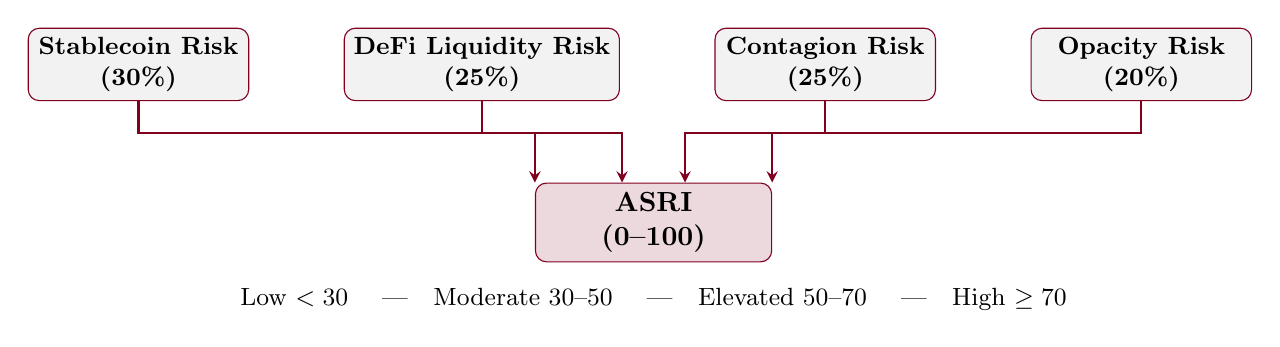
\begin{tikzpicture}[
    node distance=1cm,
    box/.style={rectangle, draw=farzullaburgundy, fill=gray!10, rounded corners, minimum width=2.8cm, minimum height=0.8cm, align=center, font=\small\bfseries},
    mainbox/.style={rectangle, draw=farzullaburgundy, fill=farzullaburgundy!15, rounded corners, minimum width=3cm, minimum height=1cm, align=center, font=\normalsize\bfseries},
    arrow/.style={->, >=stealth, thick, farzullaburgundy}
]
% Sub-indices
\node[box] (scr) {Stablecoin Risk\\(30\%)};
\node[box, right=1.2cm of scr] (dlr) {DeFi Liquidity Risk\\(25\%)};
\node[box, right=1.2cm of dlr] (cr) {Contagion Risk\\(25\%)};
\node[box, right=1.2cm of cr] (or) {Opacity Risk\\(20\%)};

% ASRI
\node[mainbox, below=1.5cm of $(dlr)!0.5!(cr)$] (asri) {ASRI\\(0--100)};

% Arrows
\draw[arrow] (scr.south) -- ++(0,-0.4) -| (asri.north west);
\draw[arrow] (dlr.south) -- ++(0,-0.4) -| ([xshift=-0.4cm]asri.north);
\draw[arrow] (cr.south) -- ++(0,-0.4) -| ([xshift=0.4cm]asri.north);
\draw[arrow] (or.south) -- ++(0,-0.4) -| (asri.north east);

% Alert levels
\node[font=\small, below=0.2cm of asri, align=center] {Low $<30$ \quad|\quad Moderate $30$--$50$ \quad|\quad Elevated $50$--$70$ \quad|\quad High $\geq70$};
\end{tikzpicture}
\caption{ASRI Framework Architecture: Four weighted sub-indices aggregate into a normalized composite risk measure with defined alert thresholds.}
\label{fig:framework}
\end{figure*}

\subsection{Weight Selection Justification}

Sub-index weights were selected based on theoretical importance and precedent from traditional systemic risk literature:

\begin{itemize}
    \item \textbf{Stablecoin Risk (30\%)}: Stablecoins are the foundational liquidity layer for DeFi. Their failure would immediately impact all protocols dependent on stablecoin-denominated liquidity pools.

    \item \textbf{DeFi Liquidity Risk (25\%)}: Protocol concentration and leverage dynamics directly determine the ecosystem's resilience to market stress.

    \item \textbf{Contagion Risk (25\%)}: DeFi-TradFi linkages represent the primary channel through which crypto stress could affect traditional finance (and vice versa).

    \item \textbf{Opacity Risk (20\%)}: While important, opacity is an amplifying factor rather than a primary risk driver. Lower weight reflects this secondary role.
\end{itemize}

Sensitivity analysis (Section 5.3) will test robustness to alternative weight specifications.

\subsection{Stablecoin Concentration Risk (30\%)}

The Stablecoin Risk sub-index captures reserve composition vulnerabilities, peg stability, and concentration across issuers:

\begin{equation}
\text{SCR}_t = 0.4 \cdot \text{TVL}_t + 0.3 \cdot \text{Treasury}_t + 0.2 \cdot \text{HHI}_t + 0.1 \cdot \text{Vol}_t
\label{eq:stablecoin}
\end{equation}

where:

\begin{itemize}
    \item $\text{TVL}_t = \frac{\text{Stablecoin TVL}_t}{\max_{\tau \leq t}(\text{Stablecoin TVL}_\tau)}$ measures stablecoin TVL relative to historical maximum

    \item $\text{Treasury}_t = \frac{\text{T-Bill Reserves}_t}{\text{Total Stablecoin Reserves}_t}$ captures Treasury exposure concentration

    \item $\text{HHI}_t = \sum_{i=1}^{n} s_i^2$ is the Herfindahl-Hirschman Index of stablecoin market share concentration

    \item $\text{Vol}_t$ is the 30-day realized volatility of weighted-average stablecoin peg deviation
\end{itemize}

\textbf{Data Sources}: DeFi Llama (stablecoin TVL), attestation reports (reserve composition), CoinGecko (price feeds for volatility calculation).

\subsection{DeFi Liquidity Risk (25\%)}

The DeFi Liquidity sub-index captures protocol concentration, leverage dynamics, and smart contract vulnerability:

\begin{equation}
\begin{split}
\text{DLR}_t = {} & 0.35 \cdot \text{Conc}_t + 0.25 \cdot \text{TVLVol}_t \\
& + 0.20 \cdot \text{SC}_t + 0.10 \cdot \text{Flash}_t + 0.10 \cdot \text{Lev}_t
\end{split}
\label{eq:defi}
\end{equation}

where:

\begin{itemize}
    \item $\text{Conc}_t$ is the HHI of TVL across top-10 DeFi protocols

    \item $\text{TVLVol}_t$ is the 30-day volatility of total DeFi TVL

    \item $\text{SC}_t$ is a composite smart contract risk score based on audit status, time since deployment, and exploit history

    \item $\text{Flash}_t$ measures flash loan volume spikes relative to 90-day average

    \item $\text{Lev}_t$ captures 30-day change in aggregate leverage ratios across lending protocols
\end{itemize}

\textbf{Data Sources}: DeFi Llama (TVL, protocol data), Token Terminal (flash loan data), DefiSafety (audit scores).

\subsection{Contagion Risk (25\%)}

The Contagion Risk sub-index quantifies DeFi-TradFi linkage intensity and cross-market transmission channels:

\begin{equation}
\begin{split}
\text{CR}_t = {} & 0.30 \cdot \text{RWA}_t + 0.25 \cdot \text{Bank}_t \\
& + 0.20 \cdot \text{Link}_t + 0.15 \cdot \text{Corr}_t + 0.10 \cdot \text{Bridge}_t\,
\end{split}
\label{eq:contagion}
\end{equation}

where:

\begin{itemize}
    \item $\text{RWA}_t$ is the 30-day growth rate of tokenized real-world asset TVL

    \item $\text{Bank}_t$ is a normalized score of bank crypto exposure from regulatory filings (OCC, ECB)

    \item $\text{Link}_t$ measures stablecoin flows to TradFi-connected entities

    \item $\text{Corr}_t$ is the 30-day rolling correlation between BTC/ETH and S\&P 500

    \item $\text{Bridge}_t$ is a composite of cross-chain bridge volume and recent exploit frequency
\end{itemize}

\textbf{Data Sources}: RWA.xyz (tokenized assets), DeFi Llama (bridge data), FRED (equity indices), regulatory filings.

\subsection{Regulatory Opacity Risk (20\%)}

The Opacity Risk sub-index assesses transparency deficits and regulatory arbitrage exposure:

\begin{equation}
\begin{split}
\text{OR}_t = {} & 0.25 \cdot \text{Unreg}_t + 0.25 \cdot \text{Multi}_t \\
& + 0.20 \cdot \text{Cust}_t + 0.15 \cdot \text{Sent}_t + 0.15 \cdot \text{Trans}_t\,
\end{split}
\label{eq:opacity}
\end{equation}

where:

\begin{itemize}
    \item $\text{Unreg}_t$ is the ratio of unregulated to regulated platform volume

    \item $\text{Multi}_t$ captures multi-issuer stablecoin scheme exposure

    \item $\text{Cust}_t$ is custody concentration in non-audited jurisdictions

    \item $\text{Sent}_t$ is regulatory sentiment score from NLP analysis of SEC/ESRB/FSB announcements

    \item $\text{Trans}_t$ is a composite transparency score based on reserve attestation frequency and coverage
\end{itemize}

\textbf{Data Sources}: Regulatory filings, news APIs (GDELT), attestation calendars, manual tracking.

\subsection{Aggregate ASRI Calculation}

The final ASRI is computed as a weighted sum of normalized sub-indices:

\begin{equation}
\text{ASRI}_t = 0.30 \cdot \text{SCR}_t + 0.25 \cdot \text{DLR}_t + 0.25 \cdot \text{CR}_t + 0.20 \cdot \text{OR}_t
\label{eq:asri}
\end{equation}

Normalization uses min-max scaling over the historical sample to produce a 0--100 index:

\begin{equation}
\text{ASRI}^{\text{norm}}_t = 100 \times \frac{\text{ASRI}_t - \min_{\tau}(\text{ASRI}_\tau)}{\max_{\tau}(\text{ASRI}_\tau) - \min_{\tau}(\text{ASRI}_\tau)}
\end{equation}

\textbf{Alert Thresholds}:
\begin{itemize}
    \item $\text{ASRI} < 30$: Low systemic risk
    \item $30 \leq \text{ASRI} < 50$: Moderate systemic risk
    \item $50 \leq \text{ASRI} < 70$: Elevated systemic risk
    \item $\text{ASRI} \geq 70$: High systemic risk
\end{itemize}

\section{Data and Implementation}

\subsection{Data Sources}

Table~\ref{tab:datasources} summarizes the data sources for each ASRI component.

\begin{table*}[t]
\centering
\caption{ASRI Data Sources by Sub-Index}
\label{tab:datasources}
\small
\begin{tabularx}{\textwidth}{lXlll}
\toprule
\textbf{Sub-Index} & \textbf{Component} & \textbf{Source} & \textbf{Frequency} & \textbf{Tier} \\
\midrule
\multirow{4}{*}{Stablecoin Risk}
& TVL & DeFi Llama & Daily & 1 \\
& Treasury Reserves & Attestation Reports & Monthly & 2 \\
& Market Share & CoinGecko & Daily & 1 \\
& Peg Volatility & CoinGecko & Daily & 1 \\
\midrule
\multirow{5}{*}{DeFi Liquidity}
& Protocol TVL & DeFi Llama & Daily & 1 \\
& Flash Loan Volume & Token Terminal & Daily & 1 \\
& Smart Contract Scores & DefiSafety & Weekly & 2 \\
& Leverage Ratios & DeFi Llama & Daily & 1 \\
& Bridge Volume & DeFi Llama & Daily & 1 \\
\midrule
\multirow{5}{*}{Contagion Risk}
& RWA TVL & RWA.xyz / DeFi Llama & Daily & 1 \\
& Bank Exposure & OCC/ECB Filings & Quarterly & 2 \\
& TradFi Linkages & On-chain Analysis & Weekly & 2 \\
& Equity Correlation & FRED/Yahoo Finance & Daily & 1 \\
& Bridge Exploits & DeFi Llama & Daily & 1 \\
\midrule
\multirow{5}{*}{Opacity Risk}
& Platform Regulation & Manual Tracking & Weekly & 2 \\
& Custody Concentration & Public Disclosures & Monthly & 2 \\
& Regulatory Sentiment & GDELT/SEC Filings & Daily & 2 \\
& Attestation Frequency & Calendar Tracking & Daily & 2 \\
& Transparency Scores & DefiSafety & Weekly & 2 \\
\bottomrule
\end{tabularx}
\end{table*}

\textbf{Tier 1} sources provide daily automated API access; \textbf{Tier 2} sources require manual collection, web scraping, or have lower update frequency.

\subsection{Data Quality Framework}

Missing data is handled according to the following protocol:

\begin{itemize}
    \item \textbf{Daily data gaps ($<$ 3 days)}: Linear interpolation with confidence score 0.7
    \item \textbf{Extended gaps (3--7 days)}: Forward-fill with confidence score 0.5
    \item \textbf{Gaps $>$ 7 days}: Flag as unreliable; exclude from ASRI calculation until fresh data available
\end{itemize}

Data lag assumptions follow the $t-1$ convention: values observed at midnight UTC on date $t$ are attributed to ASRI$_{t-1}$ to avoid look-ahead bias.

\subsection{Technical Architecture}

The ASRI system architecture comprises four layers:

\begin{enumerate}
    \item \textbf{Ingestion Layer}: Python-based API clients and web scrapers fetch data from sources
    \item \textbf{Normalization Layer}: Raw data undergoes unit normalization, gap-filling, and validation
    \item \textbf{Computation Layer}: Sub-indices calculated using Equations~\ref{eq:stablecoin}--\ref{eq:opacity}; aggregate ASRI computed via Equation~\ref{eq:asri}
    \item \textbf{Publication Layer}: FastAPI REST endpoints serve current and historical ASRI values; React dashboard provides visualization
\end{enumerate}

Figure~\ref{fig:pipeline} illustrates the data flow through these layers.

\begin{figure}[ht]
\centering
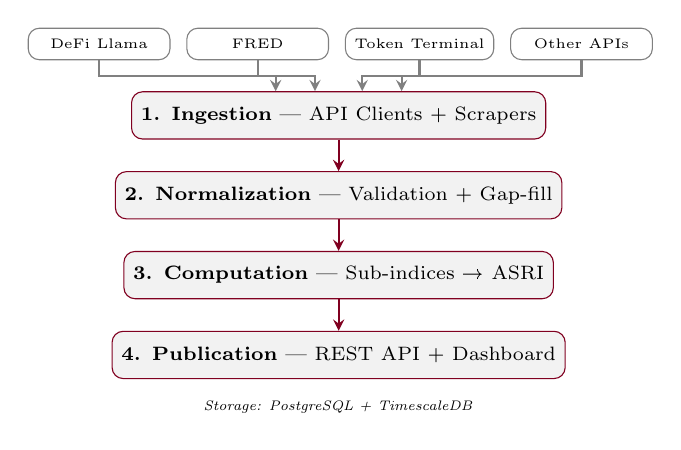
\begin{tikzpicture}[
    node distance=0.5cm,
    layer/.style={rectangle, draw=farzullaburgundy, fill=gray!10, rounded corners, minimum width=3cm, minimum height=0.6cm, align=center, font=\scriptsize},
    source/.style={rectangle, draw=gray, fill=white, rounded corners, minimum width=1.8cm, minimum height=0.4cm, align=center, font=\tiny},
    arrow/.style={->, >=stealth, thick, farzullaburgundy}
]
% Data Sources
\node[source] (dl) {DeFi Llama};
\node[source, right=0.2cm of dl] (fred) {FRED};
\node[source, right=0.2cm of fred] (tt) {Token Terminal};
\node[source, right=0.2cm of tt] (other) {Other APIs};

% Layers
\node[layer, below=0.6cm of $(fred)!0.5!(tt)$] (ingest) {\textbf{1. Ingestion} | API Clients + Scrapers};
\node[layer, below=0.4cm of ingest] (norm) {\textbf{2. Normalization} | Validation + Gap-fill};
\node[layer, below=0.4cm of norm] (comp) {\textbf{3. Computation} | Sub-indices → ASRI};
\node[layer, below=0.4cm of comp] (pub) {\textbf{4. Publication} | REST API + Dashboard};

% Arrows from sources
\draw[arrow, gray] (dl.south) -- ++(0,-0.2) -| ([xshift=-0.8cm]ingest.north);
\draw[arrow, gray] (fred.south) -- ++(0,-0.2) -| ([xshift=-0.3cm]ingest.north);
\draw[arrow, gray] (tt.south) -- ++(0,-0.2) -| ([xshift=0.3cm]ingest.north);
\draw[arrow, gray] (other.south) -- ++(0,-0.2) -| ([xshift=0.8cm]ingest.north);

% Arrows between layers
\draw[arrow] (ingest.south) -- (norm.north);
\draw[arrow] (norm.south) -- (comp.north);
\draw[arrow] (comp.south) -- (pub.north);

% Storage annotation moved below
\node[font=\tiny, below=0.15cm of pub] {\textit{Storage: PostgreSQL + TimescaleDB}};
\end{tikzpicture}
\caption{ASRI Data Pipeline: Four-layer architecture from API ingestion to public dashboard publication.}
\label{fig:pipeline}
\end{figure}

\textbf{Technology Stack}: Python 3.11+, PostgreSQL with TimescaleDB, FastAPI, React/TypeScript, Docker Compose.

Full implementation is available at \href{https://github.com/studiofarzulla/asri}{\texttt{github.com/studiofarzulla/asri}}.

\section{Proposed Validation Framework}

\textit{Note: This section outlines the validation methodology. Empirical results will be published in version 2.0.0 upon completion of historical data reconstruction.}

\subsection{Backtesting Strategy}

The ASRI will be validated against the period January 1, 2020 through December 31, 2025, capturing multiple stress events with distinct characteristics:

\begin{table}[H]
\centering
\caption{Historical Crisis Events for ASRI Validation}
\label{tab:crises}
\small
\begin{tabular}{ll}
\toprule
\textbf{Event} & \textbf{Date} \\
\midrule
COVID Market Crash & March 2020 \\
Terra/Luna Collapse & May 2022 \\
Celsius/3AC Contagion & June 2022 \\
FTX Bankruptcy & November 2022 \\
SVB Banking Crisis & March 2023 \\
\bottomrule
\end{tabular}
\end{table}

\subsection{Expected Validation Metrics}

\textbf{Precision}: Percentage of ASRI peaks (exceeding 70) that preceded or coincided with material market stress events.

\textbf{Recall}: Percentage of actual crisis events where ASRI displayed a detectable rise (increase $>$ 10 points) in the 30 days preceding the event.

\textbf{Lead Time}: Average number of days between ASRI crossing the elevated threshold (50) and crisis onset.

\textbf{False Positive Rate}: Percentage of months where ASRI exceeded 70 without subsequent market stress.

\subsection{Sensitivity Analysis}

Robustness will be tested through:

\begin{enumerate}
    \item \textbf{Weight Perturbation}: Vary each sub-index weight by $\pm$5\% and assess impact on crisis detection

    \item \textbf{Alternative Normalization}: Compare min-max scaling with z-score normalization

    \item \textbf{Regime-Specific Weights}: Test whether bull/bear/crisis regimes require different weight allocations

    \item \textbf{Walk-Forward Optimization}: Train on rolling 24-month windows and test out-of-sample
\end{enumerate}

\section{Preliminary Analysis}

\textit{Note: This section will be populated with current ASRI readings and sub-index decomposition once the data pipeline is operational. Version 2.0.0 will include:}

\begin{itemize}
    \item Current ASRI level and interpretation
    \item Sub-index breakdown and primary risk contributors
    \item Comparison to recent market events (December 2025 conditions)
    \item Visual decomposition of risk transmission channels
\end{itemize}

For live dashboard access (when available): \href{https://resurrexi.io/asri/}{\texttt{resurrexi.io/asri/}}

\section{Discussion}

\subsection{Theoretical Implications}

The ASRI framework makes three contributions to the systemic risk literature:

First, it extends network-based contagion models \citep{battiston2012debtrank} to accommodate the permissionless composability characteristic of DeFi. Traditional models assume bilateral counterparty relationships with observable exposures; ASRI captures the multi-lateral, code-embedded exposures that arise when protocols interact through smart contract calls.

Second, it formalizes the DeFi-TradFi transmission channel through stablecoin reserve composition. As stablecoins have accumulated significant Treasury positions, they create a direct link between Federal Reserve monetary policy and DeFi liquidity conditions---a channel absent from existing crypto risk measures.

Third, it operationalizes regulatory opacity as a quantifiable risk factor. While traditional finance assumes regulatory disclosure requirements, crypto markets feature substantial opacity about custody arrangements, reserve composition, and counterparty relationships. The Opacity sub-index provides a systematic framework for incorporating this uncertainty into risk assessment.

\subsection{Practical Applications}

\textbf{Portfolio Risk Management}: Institutional crypto allocators can use ASRI as a risk overlay, reducing exposure when systemic risk is elevated and increasing allocation during low-risk periods.

\textbf{Regulatory Monitoring}: Central banks and financial stability authorities can incorporate ASRI into macroprudential surveillance dashboards to monitor DeFi-TradFi interconnection dynamics.

\textbf{Protocol Governance}: DeFi protocols can use sub-index components to assess their contribution to systemic risk and adjust parameters (e.g., collateral ratios, withdrawal limits) accordingly.

\textbf{Research Applications}: The ASRI time series will provide a standardized benchmark for academic research on crypto market dynamics, enabling cross-study comparisons.

\subsection{Limitations}

\textbf{Data Availability}: Several components (Tier 2 sources) require manual collection or have limited historical depth. Enterprise APIs (TRM Labs, Chainalysis) that would improve coverage are cost-prohibitive for academic research.

\textbf{Historical Reconstruction}: DeFi data prior to 2021 is sparse, requiring proxy indicators and interpolation that reduce confidence in early-period ASRI values.

\textbf{Model Specification Uncertainty}: Weight allocation reflects theoretical judgment rather than empirical optimization. Walk-forward analysis (Section 5.3) will assess whether data-driven weights outperform.

\textbf{Regulatory Dynamics}: The rapidly evolving regulatory landscape may require periodic recalibration of the Opacity sub-index as disclosure requirements change.

\section{Conclusion}

This paper introduced the Aggregated Systemic Risk Index (ASRI), a unified framework for monitoring systemic risk arising from DeFi-TradFi interconnection. The index comprises four weighted sub-indices---Stablecoin Risk, DeFi Liquidity Risk, Contagion Risk, and Regulatory Opacity Risk---designed to capture risk transmission channels absent from traditional systemic risk measures.

The methodology presented here establishes the theoretical and computational foundation for a live risk monitoring system. Version 2.0.0 will extend this work with:

\begin{enumerate}
    \item Backtesting results against 2020--2025 historical data
    \item Validation metrics for crisis detection performance
    \item Sensitivity analysis of weight specifications
    \item Comparative analysis against existing risk indices
\end{enumerate}

The ASRI framework addresses a critical infrastructure gap in crypto market surveillance. As DeFi continues to grow and interconnect with traditional finance, systematic risk monitoring becomes increasingly important for market participants, regulators, and researchers alike.

\textbf{Live Dashboard}: \href{https://resurrexi.io/asri/}{\texttt{resurrexi.io/asri/}}

\textbf{Code Repository}: \href{https://github.com/studiofarzulla/asri}{\texttt{github.com/studiofarzulla/asri}}

% ============================================================================
% REFERENCES
% ============================================================================

\clearpage
\onecolumn

\bibliography{references}

% ============================================================================
% APPENDICES
% ============================================================================

\appendix

\section{API Documentation Summary}

Table~\ref{tab:apis} provides endpoint documentation for primary data sources.

\begin{table*}[h]
\centering
\caption{Primary API Endpoints}
\label{tab:apis}
\small
\begin{tabularx}{\textwidth}{lXll}
\toprule
\textbf{Source} & \textbf{Endpoint} & \textbf{Rate Limit} & \textbf{Authentication} \\
\midrule
DeFi Llama & \texttt{api.llama.fi/v2/tvl} & 300/5min & None \\
DeFi Llama & \texttt{stablecoins.llama.fi/stablecoins} & 300/5min & None \\
FRED & \texttt{api.stlouisfed.org/fred/series} & None & API Key \\
CoinGecko & \texttt{api.coingecko.com/api/v3} & 10-50/min & API Key (Pro) \\
Token Terminal & \texttt{api.tokenterminal.com/v2} & Varies & API Key \\
\bottomrule
\end{tabularx}
\end{table*}

\section{Sub-Index Calculation Code}

Python implementation of sub-index formulas is available in the repository at \texttt{src/asri/signals/calculator.py}. Key functions:

\begin{verbatim}
def calculate_stablecoin_risk(
    tvl_ratio: float,
    treasury_weight: float,
    hhi_concentration: float,
    peg_volatility: float
) -> float:
    return (
        0.4 * tvl_ratio +
        0.3 * treasury_weight +
        0.2 * hhi_concentration +
        0.1 * peg_volatility
    )
\end{verbatim}

Full implementation: \href{https://github.com/studiofarzulla/asri}{\texttt{github.com/studiofarzulla/asri}}

\section{Historical Crisis Event Details}

\textbf{Terra/Luna Collapse (May 2022)}: UST algorithmic stablecoin depegged due to redemption spirals, eliminating \$40B in value within 72 hours. LUNA dropped from \$80 to near-zero.

\textbf{Celsius/3AC Contagion (June 2022)}: Celsius Network froze withdrawals; Three Arrows Capital defaulted on loans. Combined losses exceeded \$10B, triggering margin calls across crypto lending platforms.

\textbf{FTX Bankruptcy (November 2022)}: FTX and Alameda Research filed for bankruptcy after liquidity crisis. Opaque counterparty relationships propagated losses across the ecosystem.

\end{document}
